\documentclass[aspectratio=1610]{beamer}

\title{ZK-Snark i njegova primena za zaštitu privatnosti u Blockchain mrežama}
\author{Matija Stanković}
\date{\today}

\usetheme[sectionpage=none]{wildcat}

\begin{document}

\begin{frame}
\titlepage
\end{frame}

\begin{frame}{Plan izlaganja}
\tableofcontents
\end{frame}

\section{Kratko podsećanje}

\begin{frame}{Dokazi nultog znanja}
\begin{block}{Osnovna ideja}
Dokazi nultog znanja omogućavaju da se potvrdi istinitost tvrdnje bez otkrivanja informacija koje su korišćene za njeno dokazivanje.
\end{block}

\begin{itemize}
    \item dokazivač poseduje određenu tajnu informaciju
    \item verifikator proverava tvrdnju
    \item sama tajna ostaje skrivena
\end{itemize}
\end{frame}

\begin{frame}{Privatnost i proverljivost}
U mnogim sistemima istovremeno želimo:

\bigskip

\begin{columns}

\begin{column}{0.48\textwidth}
\begin{block}{Privatnost}
Zaštitu osetljivih podataka korisnika.
\end{block}
\end{column}

\begin{column}{0.48\textwidth}
\begin{block}{Proverljivost}
Mogućnost nezavisne provere ispravnosti sistema.
\end{block}
\end{column}

\end{columns}

\bigskip

Dokazi nultog znanja predstavljaju jedan od načina da se ova dva zahteva istovremeno zadovolje.
\end{frame}

\begin{frame}{Problem interaktivnosti}
Klasični protokoli dokaza nultog znanja često zahtevaju više koraka komunikacije između učesnika.

\bigskip

\begin{center}
Dokazivač \(\longleftrightarrow\) Verifikator
\end{center}

\bigskip

\begin{itemize}
    \item razmena više poruka
    \item aktivno učešće obe strane
    \item manja praktičnost u distribuiranim sistemima
\end{itemize}
\end{frame}

\begin{frame}
\centering
\vfill

{\Huge Uvod u zk-SNARK}

\vfill
\end{frame}

\section{Uvod u zk-SNARK}

\begin{frame}{Značenje naziva}
Naziv zk-SNARK opisuje ključne osobine sistema.

\bigskip

\begin{itemize}
    \item \textbf{Zero-Knowledge}
    \item \textbf{Succinct}
    \item \textbf{Non-Interactive}
    \item \textbf{Argument of Knowledge}
\end{itemize}

\bigskip
\end{frame}

\begin{frame}{Javna tvrdnja, svedok i relacija}
U formalnom opisu razlikujemo:

\bigskip

\begin{itemize}
    \item \(x\) -- javnu tvrdnju
    \item \(w\) -- svedoka
    \item \(R\) -- relaciju
\end{itemize}

\bigskip

\[
R(x,w)=1
\]

\bigskip

Dokazivač pokazuje da poznaje odgovarajući svedok \(w\), bez njegovog otkrivanja.
\end{frame}

\begin{frame}{Tri osnovna algoritma}

\[
(pk,vk)\leftarrow Setup()
\]

\[
\pi\leftarrow Prove(pk,x,w)
\]

\[
Verify(vk,x,\pi)=1
\]

\bigskip

\begin{itemize}
    \item Setup generiše parametre sistema
    \item Prove konstruiše dokaz
    \item Verify proverava dokaz
\end{itemize}

\end{frame}

\begin{frame}{Tok rada zk-SNARK sistema}

\begin{center}
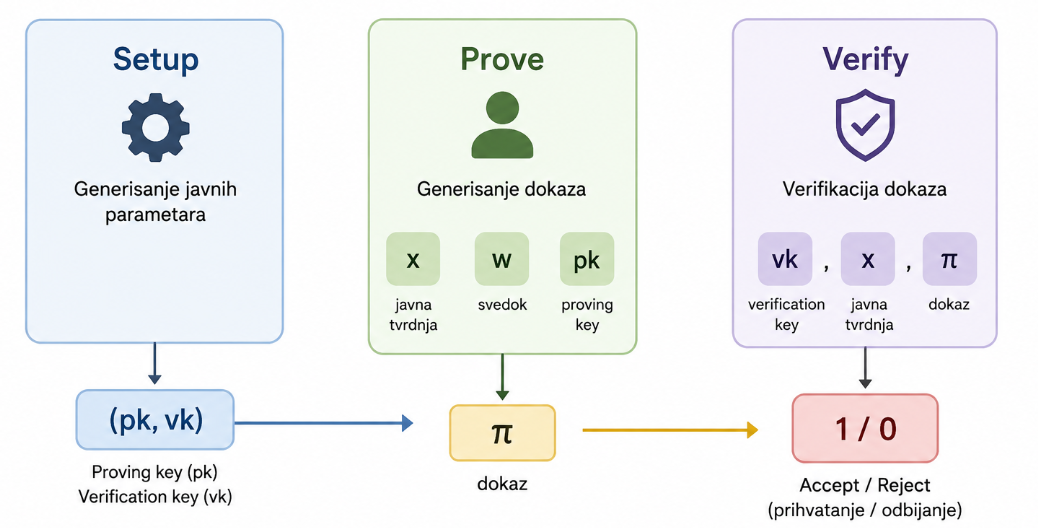
\includegraphics[width=0.75\textwidth]{../../2026_seminarski/images/zk-Snark/zkSnarkWorkFlow.png}
\end{center}

\begin{itemize}
    \item generišu se parametri sistema
    \item dokazivač konstruiše dokaz
    \item verifikator proverava njegovu validnost
\end{itemize}

\end{frame}

\begin{frame}{Trusted setup}
Većina tradicionalnih zk-SNARK sistema zahteva inicijalnu trusted setup fazu.

\bigskip

\begin{itemize}
    \item generišu se javni parametri
    \item koriste se i tajne vrednosti
    \item tajne vrednosti moraju biti uništene nakon završetka postupka
\end{itemize}
\end{frame}

\begin{frame}{Zašto je trusted setup problem?}

\begin{block}{Potencijalni rizik}
Ako bi tajni podaci korišćeni tokom setup faze ostali dostupni, mogli bi ugroziti bezbednost sistema.
\end{block}

\bigskip

\begin{itemize}
    \item moguće je generisati lažne dokaze
    \item verifikatori ih ne bi razlikovali od validnih
    \item bezbednost sistema bila bi narušena
\end{itemize}

\end{frame}

\begin{frame}{Od problema do dokaza}
    Osnovna ideja zk-SNARK sistema može se predstaviti kroz tri koraka.
    
    \bigskip
    
    \begin{center}
    Problem
    
    \(\Downarrow\)
    
    Matematička ograničenja
    
    \(\Downarrow\)
    
    Dokaz
    \end{center}
    
    \bigskip
    
    Složeni problemi prevode se u formu pogodnu za efikasno dokazivanje.
    \end{frame}

\begin{frame}
\centering
\vfill

{\Huge Primena zk-SNARK sistema za zaštitu privatnosti u blokčejn mrežama}

\vspace{0.6cm}

{\Large Zcash}

\vfill
\end{frame}

\section{Primena zk-SNARK sistema za zaštitu privatnosti u blokčejn mrežama}

\begin{frame}{Privatnost u blokčejnu}
Transparentnost predstavlja jednu od osnovnih karakteristika blokčejn mreža.

\bigskip

Kod Bitcoina svka transakcija sadrži:

\begin{itemize}
    \item adresu pošiljaoca
    \item adresu primaoca
    \item iznos transakcije
    \item istoriju prenosa sredstava
\end{itemize}

\bigskip

Takav pristup doprinosi proverljivosti, ali može ugroziti privatnost korisnika.
\end{frame}

\begin{frame}{Primer Bitcoin transakcije}
Posmatrajmo jednostavan primer.

\bigskip

Ivana želi da pošalje Matiji \(1\,\mathrm{BTC}\).

\bigskip

\begin{itemize}
    \item transakcija se šalje mreži
    \item mreža proverava njenu validnost
    \item nakon potvrde Matija postaje vlasnik sredstava
\end{itemize}

\bigskip

Podaci o transakciji ostaju javno dostupni svim učesnicima mreže.
\end{frame}

\begin{frame}{Šta mreža proverava?}
Da bi transakcija bila prihvaćena, potrebno je proveriti:

\begin{itemize}
    \item da pošiljalac poseduje sredstva
    \item da sredstva nisu prethodno potrošena
    \item da je očuvana ukupna vrednost
    \item da su ispoštovana pravila sistema
\end{itemize}

\bigskip

Kod Bitcoina se ove provere zasnivaju na javno dostupnim podacima.
\end{frame}

\begin{frame}{Klasična blokčejn transakcija}

\begin{center}
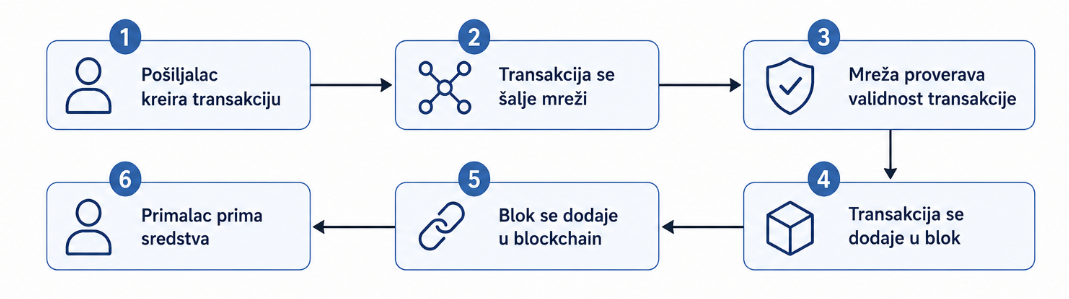
\includegraphics[width=0.78\textwidth]{../../2026_seminarski/images/zk-Snark/blockchainTransactionFlow.png}
\end{center}

\begin{itemize}
    \item svi podaci o transakciji su javni
    \item validnost se proverava direktnim uvidom u podatke
    \item transparentnost je potpuna
\end{itemize}

\end{frame}

\begin{frame}{Ideja Zcash sistema}
Zcash je razvijen sa ciljem zaštite privatnosti korisnika.

\bigskip

Kod zaštićenih transakcija mogu ostati skriveni:

\begin{itemize}
    \item identitet pošiljaoca
    \item identitet primaoca
    \item iznos transakcije
\end{itemize}

\bigskip

Istovremeno, mreža mora moći da proveri validnost transakcije.
\end{frame}

\begin{frame}{Bitcoin i Zcash}

\begin{center}
\begin{tabular}{|l|c|c|}
\hline
\textbf{Podatak} & \textbf{Bitcoin} & \textbf{Zcash} \\
\hline
Pošiljalac & vidljiv & može biti skriven \\
\hline
Primalac & vidljiv & može biti skriven \\
\hline
Iznos & vidljiv & može biti skriven \\
\hline
Validnost & proverljiva & proverljiva \\
\hline
\end{tabular}
\end{center}

\bigskip

Zcash koristi zaštićene adrese koje omogućavaju viši nivo privatnosti.
\end{frame}

\begin{frame}{Naizgled nerešiv problem}

\begin{center}
\Large

Ako su pošiljalac, primalac i iznos skriveni,

\vspace{0.5cm}

kako mreža zna da je transakcija validna?

\end{center}

\vspace{0.5cm}

Odgovor daje zk-SNARK dokaz.
\end{frame}

\begin{frame}{Očuvanje vrednosti}

Jedno od osnovnih pravila sistema jeste očuvanje ukupne vrednosti transakcije.

\[
\sum v_{\text{ulaz}}=\sum v_{\text{izlaz}}
\]

\bigskip

\begin{itemize}
    \item sredstva ne mogu nastati ni iz čega
    \item sredstva ne mogu nestati
    \item ukupna vrednost mora ostati očuvana
\end{itemize}

\end{frame}

\begin{frame}{Šta zk-SNARK dokaz potvrđuje?}

zk-SNARK dokaz potvrđuje da:

\begin{itemize}
    \item pošiljalac poseduje sredstva
    \item sredstva nisu prethodno potrošena
    \item očuvana je ukupna vrednost
    \item transakcija poštuje pravila sistema.
\end{itemize}

\bigskip

Pri tome se privatni podaci ne otkrivaju.

\[
R(x,w)=1
\]

\end{frame}

\begin{frame}{Kako nastaje dokaz?}

\begin{center}

Transakcija

\vspace{0.3cm}

\(\Downarrow\)

\vspace{0.3cm}

Matematička ograničenja

\vspace{0.3cm}

\(\Downarrow\)

\vspace{0.3cm}

zk-SNARK dokaz

\end{center}

\bigskip

Mreža proverava dokaz, a ne privatne podatke korisnika.
\end{frame}

\begin{frame}{Primer Zcash transakcije}

Posmatrajmo isti primer.

\bigskip

Ivana želi da pošalje Matiji \(1\,\mathrm{ZEC}\).

\bigskip

\begin{itemize}
    \item generiše zk-SNARK dokaz
    \item transakcija se šalje mreži
    \item mreža proverava dokaz
    \item Matija postaje vlasnik sredstava.
\end{itemize}

\bigskip

Pošiljalac, primalac i iznos mogu ostati skriveni.
\end{frame}

\begin{frame}{Tok jedne Zcash transakcije}

\begin{center}
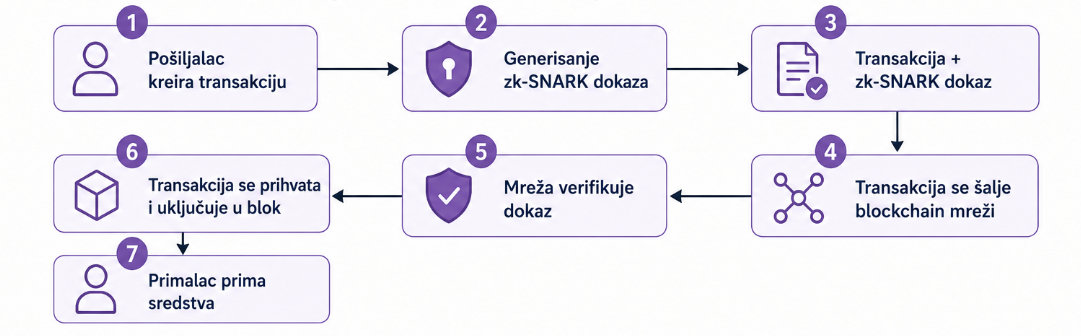
\includegraphics[width=0.78\textwidth]{../../2026_seminarski/images/zk-Snark/zkSnarkTransactionFlow.png}
\end{center}

\begin{itemize}
    \item korisnik generiše dokaz
    \item mreža proverava dokaz
    \item validna transakcija se uključuje u blok
\end{itemize}

\end{frame}

\begin{frame}{Šta verifikatori saznaju?}

Verifikatori ne moraju da znaju:

\begin{itemize}
    \item ko šalje sredstva
    \item ko prima sredstva
    \item koliki je iznos transakcije
\end{itemize}

\bigskip

Jedina informacija koju dobijaju jeste da su sva pravila sistema zadovoljena i da je transakcija validna.

\end{frame}

\begin{frame}
\centering
\vfill

{\Huge Prednosti i nedostaci}

\vfill
\end{frame}

\section{Prednosti i nedostaci}

\begin{frame}{Prednosti zk-SNARK sistema}

\begin{block}{Ključne prednosti}
\begin{itemize}
    \item mala veličina dokaza
    \item brza verifikacija
    \item visok nivo privatnosti
    \item pogodnost za blokčejn sisteme
\end{itemize}
\end{block}

\bigskip

\begin{itemize}
    \item dokazi ostaju kratki čak i za složene proračune
    \item verifikacija zahteva malo resursa
    \item privatni podaci ne moraju biti javno dostupni.
\end{itemize}

\end{frame}

\begin{frame}{Nedostaci zk-SNARK sistema}

\begin{block}{Glavna ograničenja}
\begin{itemize}
    \item trusted setup
    \item zahtevno generisanje dokaza
    \item složena implementacija.
\end{itemize}
\end{block}

\bigskip

\begin{itemize}
    \item bezbednost zavisi od pravilno sprovedenog setup-a
    \item dokazivač obavlja veliki deo računanja
    \item implementacija zahteva napredna matematička i kriptografska znanja
\end{itemize}

\end{frame}

\begin{frame}
\centering
\vfill

{\Huge Zaključak}

\vfill
\end{frame}

\section{Zaključak}

\begin{frame}{Zaključak}

\begin{block}{Glavna ideja}
zk-SNARK omogućava dokazivanje bez otkrivanja podataka na kojima se dokaz zasniva.
\end{block}

\bigskip

Kroz primer Zcash mreže videli smo da je moguće:

\begin{itemize}
    \item zaštititi privatnost korisnika
    \item sakriti detalje transakcije
    \item zadržati javnu proverljivost sistema
\end{itemize}

\bigskip

Na taj način postiže se ravnoteža između privatnosti i bezbednosti.

\end{frame}

\begin{frame}{Pogled unapred}

Jedan od najpoznatijih alternativnih pristupa predstavljaju zk-STARK sistemi.

\bigskip

Njihov cilj je da otklone neka ograničenja tradicionalnih zk-SNARK sistema, pre svega potrebu za trusted setup fazom.

\bigskip

Ipak, i oni uvode sopstvene kompromise, zbog čega se danas aktivno istražuju i razvijaju oba pristupa.

\end{frame}

\begin{frame}
\centering

\vfill

{\Huge Hvala na pažnji!}

\vspace{1cm}

{\Large Pitanja?}

\vfill

\end{frame}

\begin{frame}{Ispitna pitanja}
\begin{enumerate}
    \item Objasniti osnovnu ideju zk-SNARK sistema i ulogu javne tvrdnje, svedoka i relacije \(R(x,w)\).

    \item Objasniti na koji način se pomoću zk-SNARK dokaza proverava validnost zaštićene Zcash transakcije.

    \item Navesti i objasniti glavne prednosti i nedostatke zk-SNARK sistema.
\end{enumerate}
\end{frame}

\end{document}
